\chapter[Geometry of Parameter-Space and Berry Phases]{Geometry of Parameter-Space and Berry Phases}\label{chap11}

\Authorline{R Parthasarathy\footnote[*]{Email:  \url{sarathy@cmi.ac.in}}}
\addtocontents{toc}{\protect\contentsline{section}{{\sl R Parthasarathy}\smallskip}{}}

\authinfo{Retired Professor, The Institute of Mathematical Sciences \\
Chennai 600 113.}

\begin{abstract}
The general formalism using the parallel transport of vectors in curved space to evaluate quantum interference effects,  developed in Ref.\ 6, is extended to revisit Berry phase by relaxing the adiabatic approximation. 
\end{abstract}
\bigskip

\centerline{\textit{\textbf{Dedication}}}
\smallskip

Prof.\ G. Ramachandran, an excellent theoretical physicist, was very simple and had clear understanding of  various branches in Theoretical Physics. His lectures on Quantum Theory of Angular Momentum  (MATSCIENCE REPORT 2, 1963) bears his  thorough understanding and clarity. He taught me the nuances of density matrix methods in nuclear  reactions in 1971 and my very first research paper has him as a coauthor along with Prof.\ V. Devanathan. I kept correspondence with him till 2019. I consider it an honour to dedicate this  article to his memorial volume.

\section{Introduction}\label{chap11-sec1}

Berry \cite{chap11-key1} has shown that a quantum mechanical system in an eigenstate $|n\rangle$ (non-degenerate), slowly transported  adiabatically around a closed curve ${\cal{C}}$ in the parameter space, by varying the parameters $R_i(t)$ in the  Hamiltonian $H(R_i(t))$, will acquire a geometrical phase $e^{i{\gamma}_{\cal{C}}}$ in addition to the familiar dynamical  phase $e^{i\int_0^T\ E_n(t)dt}$, when $H(R_i(0))=H(R_i(T))$. This additional phase, the Berry phase, arises from the  adiabatic transport of the system around the closed loop in the parameter space while the Hamiltonian returns to its  initial value. Thus, while the Hamiltonian returns to its initial value, the wave function does not and  acquires a geometric phase. 

Simon \cite{chap11-key2} identified this important geometric phase as the holonomy in a Hermitian line bundle in the parameter space. Omitting the standard derivation this phase is  
\begin{equation}
{\gamma}_n({\cal{C}})= {\oint}_{\cal{C}}\ \langle n|{\vec{\nabla}}_R|n\rangle \cdot d\vec{R}, \label{chap11-eq1}
\end{equation}
where ${\vec{\nabla}}_R$ is the gradient operator in the space of parameters. This is Berry's result. The total phase 
acquired is 
\begin{equation}
\delta W= \int_0^T\ E_n(t)dt+i{\oint}_{\cal{C}}\ \langle n|{\vec{\nabla}}_R|n\rangle \cdot d\vec{R},\label{chap11-eq2}
\end{equation}
including the dynamical phase. The second term depends on the geometry of the parameter space and hence called the 
geometric phase.  

Three generalizations on Berry phase have been made. Wilczek and Zee \cite{chap11-key3} allowed the instantaneous eigenstates to be  degenerate; Aharonov and Anandan \cite{chap11-key4} allowed the evolution to be non-adiabatic; Berry \cite{chap11-key5} made the system to return  to its original state not exactly but in a close approximation and obtained corrections to the geometric phase,  not perurbatively but iteratively. The $k$th phase approximant obtained by Berry \cite{chap11-key5} is given by 
\begin{equation}
\gamma (n)\simeq{\gamma}^{(k)}(n)\ =\ \sum_{j=0}^k\ {\gamma}_j(n)+\int_{-\infty}^{\infty}\ dt\{E_0(n,t)- E_k(n,t)\}, \label{chap11-eq3}
\end{equation}
where ${\gamma}_j(n)$ is the $j$th state Berry phase.

The results  \eqref{chap11-eq1}, \eqref{chap11-eq2} were obtained in \cite{chap11-key7} from the formalism developed by Parthasarathy, Rajasekaran and  Vasudevan \cite{chap11-key6} based on the fundamental concept of the {\it{parallel transport}} in a curved space, by interpreting  the unphysical space in \cite{chap11-key6} as the parameter space. It is the purpose now to get the result \eqref{chap11-eq3} of Berry \cite{chap11-key5}  by introducing 'warp factor' in the metric of the parameter space. The result we obtain here for  this bears close similarity with \eqref{chap11-eq3} and the difference will be stated. In Ref.6, we used a product space $R^1 \times B^n$ to evaluate the change in the phase of a quantum mechanical wave function of a particle around a  closed path. This change is due to the change in the momentum $p_A$ of the particle involving the 'parallel  displacement of this momentum vector'. This contained the gravitational and the electromagnetic phase shifts  (Aharonov-Bohm effect), hitherto treated separately, get unified. Subsequently, in Ref.7, it was shown that the  Berry phase \eqref{chap11-eq1} and \eqref{chap11-eq2}, emerged from the formalism in \cite{chap11-key6}. In adapting the formalism in \cite{chap11-key6} to calculate Berry phase,  as now one is considering the time evolution. If  the parameters in the Hamiltonian are taken to be slowly varying with time $t$ so that adiabatic approximation  can be effected, the relevant choice for the product space is $R^1\times B^n$, with $B^n$ as the space of $n$  parameters. With this choice of the total space $R^1\times B^n$, one focuses the phase acquired by a wave function  in this space. 

Before presenting the derivational details, the notion of metric in the parameter space $B^n$ and that of the  {\textit{parallel displacement}} will be given in the next section. 

\section{Metric in the parameter space $B^n$}\label{chap11-sec2}

In adapting the formalism developed in \cite{chap11-key6} to calculate Berry phase, the appropriate product manifold is $R^1  \times B^n$ where $R^1$ represents $t$ and $B^n$ is the space of $n$ parameters. The parameters are taken to be  slowly varying with time $t$ and {\it{the very act of treating $R^1$ and $B^n$ as disjoint, implements the  adiabatic approximation}}. Now we introduce a metric (classical) $g_{ij}(R)$ for $B^n$. The parameter space has  the property here $R^i(0)=R^i(T); i=1,2,\ldots n$, so that the Hamiltonian $H(R^i(t))$ returns to its initial value  after $T$ seconds. With $R^i(0)=R^i(T)$, the coordinates in the parameter space form non-Euclidean space and hence  an associated metric $g_{ij}(R)$. This is the usual classical metric in a non-Euclidean space. The specific form  of this metric is not needed here, as will be seen later.  Next, in the formalism in \cite{chap11-key6}, the parallel displacement of the momentum vector played crucial role.  
 
We are using the notion of parallel transport of the momentum vector in the following manner. The change in the  momentum vector $p_i$ along a curve, is given by 
\setcounter{equation}{3}
\begin{equation}
\delta p_i= \int_0^s \frac{\partial p_i}{\partial R^j}\ dR^j-\int_0^s\ {\Gamma}^j_{ik}p_j\ dR^k\ \equiv\ \int_0^s \frac{\partial p_i}{\partial R^j}\ dR^j-\bar{\delta}\ p_i, \label{chap11-eq4}
\end{equation}
where the first term involves the ordinary derivative part which does not contribute to $\delta W$ in \eqref{chap11-eq2} for  a closed loop and the second term involving the affine connection ${\Gamma}^j_{ik} = g^{jm}{\Gamma}_{ik,m}\  =\ \frac{1}{2}g^{jm}\{{\partial}_ig_{km}+{\partial}_kg_{im}-{\partial}_mg_{ik}\}$ with $g_{km}(R)$ as the metric  in $B^n$ and ${\partial}_i=\frac{\partial}{\partial R^i}$, describes the 'parallel transport' of the vector $p_i$  in the $B^n$ space. Thus, the second term requires the metric $g_{ij}(R)$ in our method.  

\section{Berry Phase - Adiabatic Approximation}\label{chap11-sec3}

As stated in Section \ref{chap11-sec2}, the act of treating $R^1$ and $B^n$ as disjoint, implements the adiabatic approximation.  The slow variation of the parameters $R^i(t)$ (coordinates) in the $B^n$ space makes the eigenfunctions of the  Hamiltonian to continue to be the eigenfunctions corresponding to every value of $R^i(t)$ at each instant of  time. This choice allows the use of factorisable metric for the product space $R^1\times B^n$ as 
\setcounter{equation}{4}
\begin{equation}
(dSs)^2= (dt)^2+g_{ij}(y)\ dy^idy^j,\label{chap11-eq5}
\end{equation}
where the coordinates $y^i$ of $B^n$ are identified with the parameters $R^i$. As $t$ goes from $0$ to $T$ in  $R^1$, we have in $B^n$ space, $y^i(0)$ going to $y^i(T)$. For cyclic evolution, $R^i(0)=R^i(T)\Rightarrow  y^i(0)=y^i(T)$, we obtain a loop in $B^n$ space. 

With this, the total phase acquired by a wave function for $R^1\times B^n$ corresponding to the eigenvalue  $E_n$ is (from equation 3.1 of Ref.6) with the expectation value for the $B^n$ part for the instantaneous   eigenstate $|n\rangle $ 
\begin{align}
\delta W= &\int_0^T \delta p_t dt+\langle n|{\oint}_{\cal{C}}\ \delta p_i dR^i|n\rangle , \nonumber \\
= &\int_0^T dt E_n(t)+\langle n|{\oint}_{\cal{C}}\ \delta p_i dR^i|n\rangle,\label{chap11-eq6}
\end{align}
where $p_i$ is the momentum operator in $B^n$ space. $\delta p_i$ consists of two parts (as in \eqref{chap11-eq4}); the ordinary  derivative part which does not contribute to the loop integral and the parallel transport part $\bar{\delta}p_i$    and so 
\begin{equation}
\delta W= \int_0^Tdt E_n(t)-\langle n|{\oint}_{B^n}{\bar{\delta}}p_{R^i} dR^i|n\rangle.\label{chap11-eq7}
\end{equation}
Replacing ${\bar{\delta}}p_{R^i}$ by its operator ($\hbar=1$), we obtain for the eigenvalue $E_n(t)$
\begin{equation}
\delta W= \int_0^T E_n(t)dt+i\int dR^i\ \langle n|{\nabla}_{R^i}|n\rangle, \label{chap11-eq8}
\end{equation}
which is \eqref{chap11-eq2}. In this formalism, the dynamical phase is also of geometrical origin as it comes from $R^1$. This  result was obtained in \cite{chap11-key7} in the adiabatic limit. 

\section{Relaxation of Adiabatic Approximation}\label{chap11-sec4}

In obtaining \eqref{chap11-eq7}, we have considered the total space as $R^1\times B^n$ and $(ds)^2$ for this product space in \eqref{chap11-eq5} implemented the adiabatic approximation as disjoint spaces. The adiabatic approximation is now relaxed by taking  $(ds)^2$ as non-factorisable ansatz 
\setcounter{equation}{8}
\begin{equation}
(ds)^2= (dt)^2+\left(\sum_{r=0}^k\ e^{h^{(r)}(t)}g_{ij}^{(r)}(y)\right)\ dy^idy^j,\label{chap11-eq9}
\end{equation}
where the 'warp factors' $h^{(r)}(t)$ are taken to be slowly varying with time $t$. The above choice still describes the  non-Euclidean geometry of $B^n$ space since the sum or weighted sum of metrics is also a metric. The real function $h^{(r)}(t)$  is arbitrary at this stage and will be chosen later. The non-vanishing connection coefficients for the above warped product  space, denoted by $\bigtriangleup$, are given by 
\begin{align}
{\bigtriangleup}^{(r) t}_{ij}&= -\frac{1}{2}\ e^{h^{(r)}(t)}\ \frac{dh^{(r)}(t)}{dt}\ g_{ij}^{(r)}, \nonumber \\
{\bigtriangleup}^{(r) i}_{tj}&= \frac{1}{2}\ \frac{dh^{(r)}(t)}{dt}\ {\delta}^i_j, \nonumber \\
{\bigtriangleup}^{(r) i}_{j\ell}&= {\Gamma}^{(r) i}_{j\ell},\label{chap11-eq10}
\end{align}
where ${\Gamma}^{(r) i}_{j\ell}=\frac{1}{2}g^{(r)\ell m}\ \{{\partial}_jg^{(r)}_{\ell m}+{\partial}_{\ell}g^{(r)}_{jm} 
-{\partial}_mg^{(r)}_{j\ell}\}$, the connections for $g_{ij}^{(r)}$. 

The 'momentum' of the particle under consideration in this warped product space is 
\begin{align}
p_A &= mg_{AB}\ \frac{dz^B}{ds}\ ;\ z^A\ =\ (t,y^i), \nonumber \\
p_t &= m\ \frac{dt}{ds}, \nonumber \\
p_i &= m\sum_{r=0}^k\ e^{h^{(r)}(t)}g_{ij}^{(r)}\frac{dy^j}{ds}=\sum_{r=0}^k p_i^{(r)}; p_i^{(r)}=me^{h^{(r)}(t)}
g_{ij}^{(r)}\frac{dy^j}{ds}.\label{chap11-eq11}
\end{align}

Now, the second term in \eqref{chap11-eq7} (the parallel transport part) for the non-factorisable case of \eqref{chap11-eq9} becomes, upon  observing the sum over $i$ in the second term in \eqref{chap11-eq7} has to be enlarged to a sum over $A=(t,i)$ as the warp  factor in \eqref{chap11-eq9} (in front of $dy^idy^j$) involves $t$ through $h^{(r)}(t)$,  
\begin{align}
\oint {\bar{\delta}}p_A\ dz^A= &-\oint dz^A\int_0^s{\bigtriangleup}^B_{AC}p_B\ \frac{dz^C}{ds} ds, \nonumber \\
= &-\oint dt\int_0^s{\bigtriangleup}^B_{tC}p_B\frac{dz^C}{ds}ds-\oint dy^i\int_0^s{\bigtriangleup}^B_{iC}p_B
\frac{dz^C}{ds}ds,\label{chap11-eq12}
\end{align}
The first term in \eqref{chap11-eq12} is expanded using \eqref{chap11-eq10} and \eqref{chap11-eq11}, and observing ${\bigtriangleup}^t_{tC}=0$, this term becomes 
\begin{align}
-\oint dt\int_0^s{\bigtriangleup}^B_{tC}p_B dz^C= &-\oint dt\int_0^s {\bigtriangleup}^i_{tC}\ p_i\ dz^C, \nonumber \\
= &-\oint dt\int_0^s {\bigtriangleup}^i_{tj}\ p_i\ dy^j, \nonumber \\
= &-\oint dt\int_0^s\sum_{r=0}^k\frac{m}{2}\left(\frac{d}{dt}h^{(r)}(t)\right) \nonumber \\
& \qquad \sum_{k'=0}^ke^{h^{(k')}(t)}g_{i\ell}^{(k')} \frac{dy^{\ell}}{ds}\frac{dy^i}{ds}ds. \label{chap11-eq13}
\end{align}
From \eqref{chap11-eq9}, dividing by $(ds)^2$, we have $ {\sum}_{k'=0}^ke^{h^{(k')}(t)}g_{i\ell}^{(k')}\ 
\frac{dy^{\ell}}{ds}\frac{dy^i}{ds}=1-\left(\frac{dt}{ds}\right)^2$ and so \eqref{chap11-eq13} becomes 
\begin{align}
-\oint dt\int_0^s{\bigtriangleup}^B_{tC}p_Bdz^C= &-\oint dt\frac{m}{2}\int_0^s \sum_{r=0}^k \left(\frac{d}{dt}
h^{(r)}(t)\right)\ \left(1-\left(\frac{dt}{ds}\right)^2\right) ds, \nonumber \\
\simeq & -\frac{m}{2}\oint dt \int_0^s\sum_{r=0}^k\ \left(\frac{d}{dt}h^{(r)}(t)\right)\ ds,\label{chap11-eq14}
\end{align}
where in obtaining the last step we have neglected the contribution from $\left(\frac{dt}{ds}\right)^2$ as this 
factor is $\frac{p_t^2}{m^2}$ from \eqref{chap11-eq11} which along with the prefactor $\frac{d}{dt}h^{(r)}(t)$, for slow 
variation of $h^{(r)}(t)$ will be very small. 

We have not specified the real function $h^{(r)}(t)$ till now. We choose this function to correspond to the initial
eigenstate $|n\rangle$ as 
\begin{equation}
h^{(r)}(t)= \frac{2}{m}\int^t E_r(n,t') dt'.\label{chap11-eq15}
\end{equation}
For the $k$th instantaneous energy state, the sum over $r$ in \eqref{chap11-eq14} picks out the $k$th energy eigenvalue by  introducing ${\delta}_{rk}$, so that following \cite{chap11-key2}, we find 
\begin{equation}
-\oint dt \int_0^s {\bigtriangleup}^B_{tC}p_B\ dz^C\simeq -\int_0^T\ E_k\left(n,\frac{s}{T}\right) ds. \label{chap11-eq16}
\end{equation}
Here the correspondence with the instantaneous energy in the $k$th iterated Hamiltonian used by Berry \cite{chap11-key5} is made. However, they are not the same as we do not use explicitly a Hamiltonian here.

The second term in \eqref{chap11-eq12} is expanded as  
\begin{align}
	-\oint dy^i\int_0^s{\bigtriangleup}^B_{iC} p_B\frac{dz^C}{ds}ds= &-\oint dy^i\left( \int_0^s {\bigtriangleup}^B_{it}
	p_B dt+\int_0^s{\bigtriangleup}^B_{ij}p_B dy^j\right), \nonumber \\
	= &-\oint dy^i\left(\int_0^s{\bigtriangleup}^j_{it}p_j dt+\int_0^s{\bigtriangleup}^t_{ij}p_t dy^j \right. \nonumber \\
	& \qquad \qquad \qquad \quad \left.+\int_0^s {\bigtriangleup}^{\ell}_{ij}p_{\ell} dy^j\right),\label{chap11-eq17}
\end{align}
since ${\bigtriangleup}^t_{it}=0$. Substituting ${\bigtriangleup}^j_{it}, {\bigtriangleup}^t_{ij},{\bigtriangleup}^{\ell}
_{ij}$ from \eqref{chap11-eq10} and using \eqref{chap11-eq11}, we find 
\begin{align}
	-\oint dy^i & \int_0^s{\bigtriangleup}^B_{iC} p_B\frac{dz^C}{ds}ds\nonumber \\
	= &-\oint dy^i \left[ \frac{m}{2}\int_0^s \sum_{r=0}^k\frac{dh^{(r)}}{dt}\ e^{h^{(r)}(t)}g^{(r)}_{ij}\frac{dy^j}{ds} dt -\frac{m}{2}\int_0^s\right.\nonumber\\ 
	& \qquad \qquad  \left.\sum_{r=0}^k e^{h^{(r)}(t)}\frac{dh^{(r)}}{dt}g^{(r)}_{ij} dy^j\frac{dt}{ds} + \int_0^s\sum_{r=0}^k{\Gamma}^{(r) \ell}_{ij}p_{\ell}^{(r)} dy^j \right], \nonumber \\
	= &-\oint dy^i\int_0^s\sum_{r=0}^k {\Gamma}^{(r)\ell}_{ij}p^{(r)}_{\ell}\frac{dy^j}{ds} ds
	= -\oint dy^i\sum_{r=0}^k \bar{\delta} p_i^{(r)}, \label{chap11-eq18}
\end{align}
where the $h^{(r)}(t)$ terms cancel each other (this is important so as to preserve the sum over $r$ from $0$ to $k$ for  the last step) and in the last step, $\bar{\delta}p_i$ is  obtained with parallel transport corresponding to $g^{(r)}_{ij}$ only with the sum over $r$ from $0$ to $k$.  Compared with the second term in \eqref{chap11-eq7},  {\it{now}}, it gets two contributions \eqref{chap11-eq16} and \eqref{chap11-eq18} (with sum over $r$ in \eqref{chap11-eq18} only)   due to the warped metric in \eqref{chap11-eq9} which relaxes the adiabatic approximation.
\newpage

Replacing $\bar{\delta}p_i$ in \eqref{chap11-eq18} by its expectation value (as done in \eqref{chap11-eq8}) and including the first term in \eqref{chap11-eq7}, we  find the total phase acquired is 
\begin{equation}
\delta W=  \int_0^T dt\{E_n(t)-E_k(n,t)\} +\sum_{r=0}^k{\gamma}^{(r)}(n), \label{chap11-eq19}
\end{equation}
with
\begin{equation}
{\gamma}^{(r)}(n)= i\int dR^i\langle n|{\nabla}^{(r)}_i|n\rangle,\label{chap11-eq20}
\end{equation}
thereby agreeing with \eqref{chap11-eq3} formally.    

The formalism given in \cite{chap11-key6, chap11-key7} and adopted here is crucially dependent on the geometry of the parameter space. We have  not made explicit use of Schr\"{o}dinger equation. By replacing the momentum by its expectation value which is pertinent  for a quantum mechanical state, we are able to obtain Berry phase result. Though \eqref{chap11-eq19} agrees formally with \eqref{chap11-eq3}, they are  not the same. The reason is that while here a specific Hamiltonian (and the Schr\"{o}dinger equation) is not used, in \cite{chap11-key5}, a  Hamiltonian is used so that the $k$th approximation made in \cite{chap11-key5} is different from the one here. The difference is that in  finding ${\gamma}_j(n)$ in \cite{chap11-key5}, the off-diagonal terms are not neglected upto the $k$th iteration and these are  neglected in $H_{k+1}$. This gave the $k$th approximant \eqref{chap11-eq3} of \cite{chap11-key5}. In our case, as no Hamiltonian is explicitly used,  the phases ${\gamma}_j(n)$ involve diagonal element with $|n\rangle$. The origin of the sum over $r$ comes from the  sum over the warp factors and the $k$th approximation here corresponds to truncating the sum over $r$ to $k$. In other  words, we realize a finite sum of Berry phases in relaxing the adiabatic approximation, instead of a single Berry  phase in the adiabatic limit.   Nevertheless, the formal similarity between \eqref{chap11-eq3} and \eqref{chap11-eq19} is striking. The result here  that the geometric phase is essentially emerging from the parallel transport of momentum vector in the product space  and does not require a Hamiltonian or its associated Schr\"{o}dinger equation, has been emphasized by Mukunda and  Simon \cite{chap11-key8}.   

\section*{Acknowlegements}

The author wishes to acknowledge with thanks the useful discussions with Professor M. V. Berry and his suggestion 
to consider the relaxing of adiabatic approximation in the formalism using parallel transport of vectors in the 
product space. The author wishes to thank him for encouragement.  

\begin{thebibliography}{99}
\bibitem{chap11-key1} M. V. Berry, Proc.\ Royal.\ Soc.\ London.\ {\bf{A392}} (1984) 45.
\bibitem{chap11-key2} B. Simon, Phys.\ Rev.\ Lett.\ {\bf 51} (1983) 2167.
\bibitem{chap11-key3} F. Wilczek and A. Zee, Phys.\ Rev.\ Lett.\ {\bf 52} (1984) 2111.
\bibitem{chap11-key4} Y. Aharonov and J. Anandan, Phys.\ Rev.\ Lett.\ {\bf 58} (1987) 1593.
\bibitem{chap11-key5} M. V. Berry, Proc.\ Royal.\ Soc.\ London.\ {\bf A414} (1987) 31.  
\bibitem{chap11-key6} R. Parthasarathy, G. Rajasekaran and R. Vasudevan, Class.\ Quant.\ Gravity.\ {\bf 3} (1986) 425.
\bibitem{chap11-key7} R. Parthasarathy, G. Rajasekaran and R. Vasudevan, in {\textit{An Unified Treatment of Quantum Interference Effects}} in \textit{Selected Topics in Mathematical Physics: Professor R. Vasudevan Memorial Volume.} Eds.\ R. Sridhar, K. Srinivasa Rao and V. Lakshminarayanan; Allied Publishers Ltd., New Delhi, India, 1995.
\bibitem{chap11-key8} N. Mukunda and R. Simon, Ann.\ Phys.\ (NY).\ {\bf 228} (1993) 205, 269.
\end{thebibliography}
\vskip 0.5cm

\centerline{\includegraphics[scale=1.8]{authorsphotos/Prof_R_Parthasarathy.eps}}
\bigskip

\noindent
\textbf{Prof.\ R. Parthasarathy} did his Ph.D. from University of Madras under Prof.\ V.Devanathan. He was a faculty member of the Institute of Mathematical Sciences, Chennai. After his retirement as Senior Professor from IMSc, he has been an Adjunct Professor at Chennai Mathematical Institute, Chennai, actively pursuing teaching and research.



